\documentclass[11pt]{article}
\usepackage{natbib,mybigpackage}
\usepackage{algorithm}
%\usepackage{program}
%\usepackage{algpseudocode}
\usepackage{algorithmic}
\usepackage{listings}
\def\xbf{\mathbf{x}}
\def\zbf{\mathbf{z}}
\def\xibf{\mathbf{\xi}}
\title{Documentation: Assignment 10}
\author{Abhinav Gupta -- 150123001}
\begin{document}
\titlepage
\newpage
\begin{enumerate}
\item[Q 1] Generate 10 sample paths for the standard Brownian Motion in the time interval [0, 5]
using the recursion.W(0)=0, Mean=0, Sigma=1.
\[W(t_{i+1}) = W(t_i)+\sqrt{t_{i+1}-t_i}.Z_{i+1}\]
\end{enumerate}
\noindent{Code: R}
\begin{lstlisting}
paths<-10
count<-5000
interval<-5/count
main_sample<-matrix(0,nrow=(count+1), ncol=paths)
png("question1.png")
for(i in 1:paths){
	main_sample[1,i]<-0
	z_sample<-rnorm(count+1)
	for(j in 2:(count+1)){
		main_sample[j,i]<-main_sample[j-1,i]+((interval)^.5)*z_sample[j]
	}
}
cat("E[W(2)] = ",mean(main_sample[2001,]),"\n")
cat("E[W(5)] = ",mean(main_sample[5001,]),"\n")
matplot(main_sample,xlab="Time",ylab="Path")
\end{lstlisting}
\noindent{\textbf{Output}:}\

E[W(2)] =  -0.6676345\

E[W(5)] =  -1.040181\
\newpage
\textbf{Graph: }\
\begin{figure}[H]
\centering
\subfloat[X1]{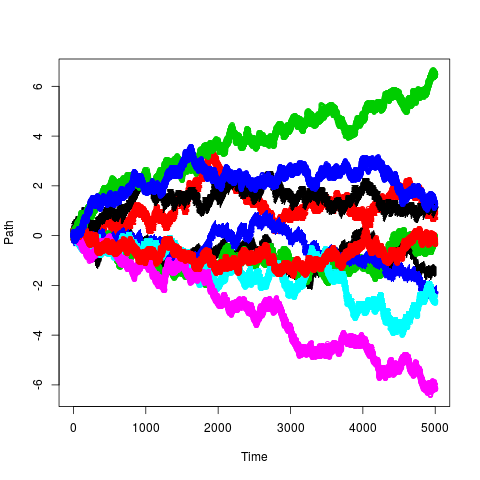
\includegraphics[width=.9\textwidth]{question1.png}}\\
\end{figure}
%----------------------------------------------------------------------------------------------------------
\newpage
\begin{enumerate}
\item[Q 2] Generate 10 sample paths for the standard Brownian Motion in the time interval [0, 5]
using the recursion. X(0)=5,Mean=0.06, Sigma=0.3.
\[X(t_{i+1}) = X(t_i)+\mu(t_{i+1}-t_{i})+\sigma\sqrt{t_{i+1}-t_i}.Z_{i+1}\]
\end{enumerate}
\noindent{Code: R}
\begin{lstlisting}
paths<-10
count<-5000
interval<-5/count
sd<-0.3
mean<-0.06
main_sample<-matrix(0,nrow=(count+1), ncol=paths)
png("question2.png")
for(i in 1:paths){
	main_sample[1,i]<-5
	z_sample<-rnorm(count+1)
	for(j in 2:(count+1)){
		main_sample[j,i]<-main_sample[j-1,i]+mean*(interval)+((interval)^.5)*z_sample[j]*sd
	}
}
cat("E[W(2)] = ",mean(main_sample[2001,]),"\n")
cat("E[W(5)] = ",mean(main_sample[5001,]),"\n")
matplot(main_sample,xlab="Time",ylab="Path")
\end{lstlisting}
\noindent{\textbf{Output}:}\

E[W(2)] =  4.725716\

E[W(5)] =  4.984472\

\newpage
\textbf{Graph: }\
\begin{figure}[H]
\centering
\subfloat[X1]{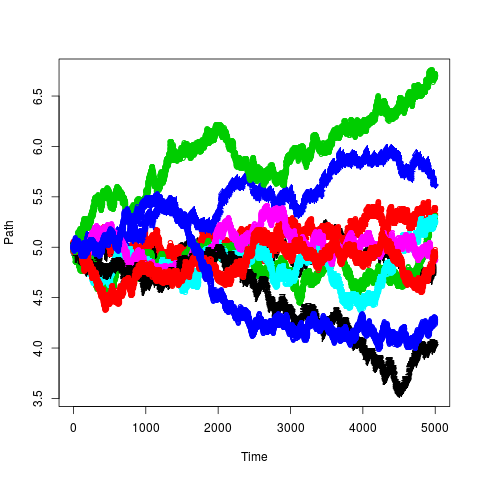
\includegraphics[width=.9\textwidth]{question2.png}}\\
\end{figure}
%---------------------------------------------------------------------------
\newpage
\begin{enumerate}
\item[Q 3] The Euler approximated recursion with time dependent mean and sigma.Y(0)=5.
\[Y(t_{i+1}) = Y(t_i)+\mu(t_i)(t_{i+1}-t_{i})+\sigma(t_i)\sqrt{t_{i+1}-t_i}.Z_{i+1}\]
\end{enumerate}
\noindent{Code: R}
\begin{lstlisting}
paths<-10
count<-5000
interval<-5/count
sigma<-function(x){
	return (0.012+0.0138*x+0.00125*x*x)
}
mean1<-function(x){
	return (0.0325-0.05*x)
}
main_sample<-matrix(0,nrow=(count+1), ncol=paths)
png("question3.png")
for(i in 1:paths){
	main_sample[1,i]<-5
	z_sample<-rnorm(count+1)
	for(j in 2:(count+1)){
		main_sample[j,i]<-main_sample[j-1,i]+mean1((j-2)*(interval))*interval+((interval)^.5)*z_sample[j]*sigma((j-2)*interval)
	}	
}
cat("E[W(2)] = ",mean(main_sample[2001,]),"\n")
cat("E[W(5)] = ",mean(main_sample[5001,]),"\n")
matplot(main_sample,xlab="Time",ylab="Path")
\end{lstlisting}
\noindent{\textbf{Output}:}

E[W(2)] =  4.960855\

E[W(5)] =  4.633403\
\newpage
\textbf{Graph: }\
\begin{figure}[H]
\centering
\subfloat[X1]{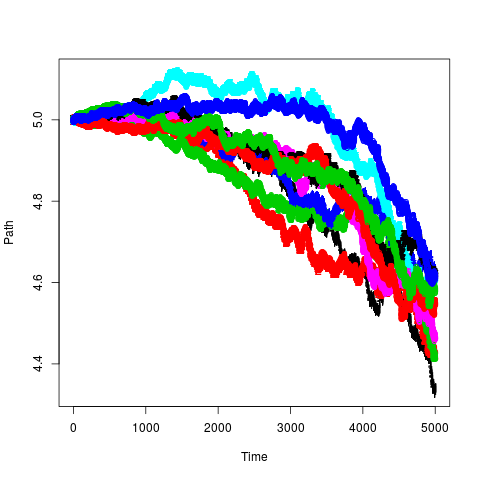
\includegraphics[width=.9\textwidth]{question3.png}}\\
\end{figure}

\end{document}